\chapter{Sprint 1: User management}
In this chapter, we will address user management as part of Sprint 1. We will examine in detail the functionalities and processes related to user management, focusing on the development and implementation stages.

The user management section involves two main actors: Users and Administrators. The two primary actions are registration and authentication. The Administrator is responsible for creating user accounts and granting access permissions to the services of our solution. Additionally, both Users and Administrators can securely manage and retrieve secrets from the vault server.
\pagebreak

\section{Analysis of Sprint 1 Requirements}
In this section, we will conduct a thorough analysis of the requirements for Sprint 1 using diagrams. We will also discuss our sprint backlog, detailing the priority items and specific tasks planned for this sprint.


\subsection{Use case diagram of "Manage users"}

The following figure (\hyperref[fig:use_case-manage_users2]{Figure \ref{fig:use_case-manage_users2}})  represents the admin ``Manage users'' detailed use case.
\begin{figure}[h]
  \center
%\hspace*{-0.9in}
  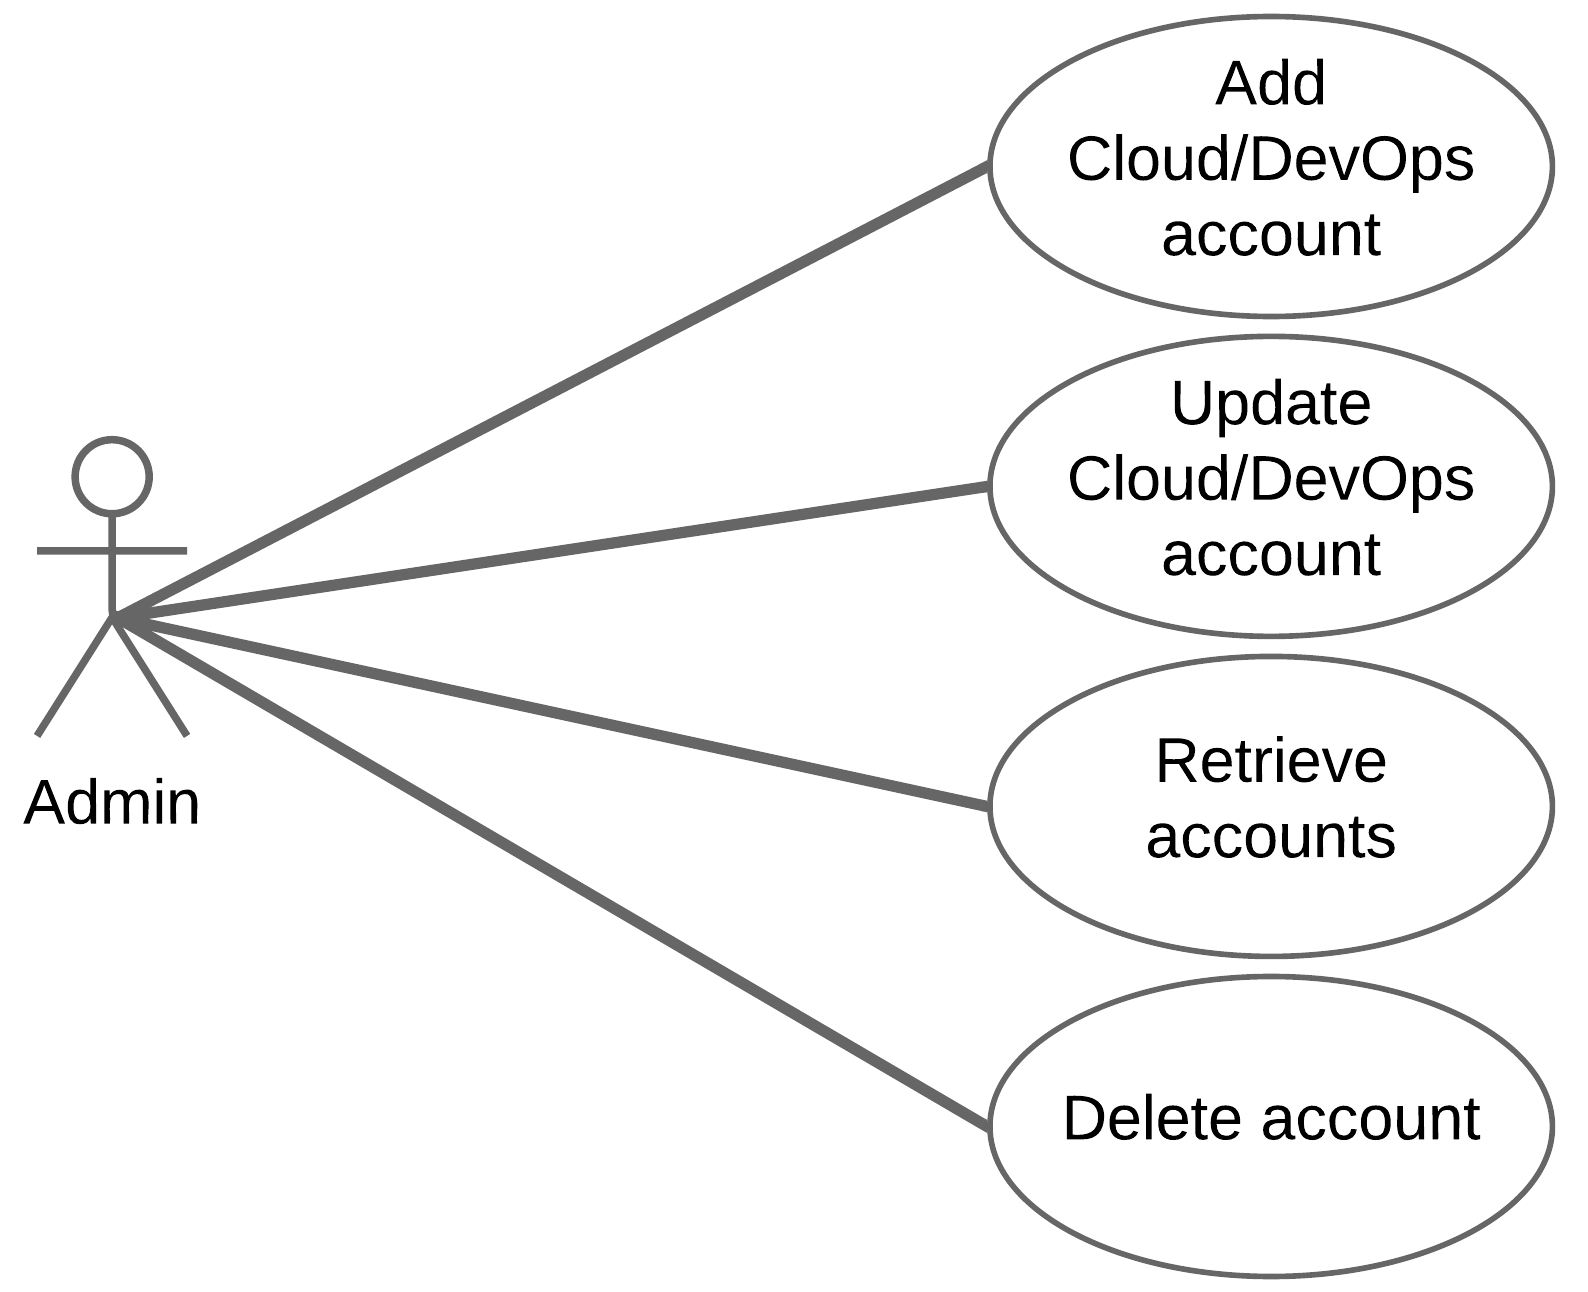
\includegraphics[width=10cm]{./chapters/sprint1/use_case-manage_users2.png}
  \caption{Manage users detailed use case diagram}
  \label{fig:use_case-manage_users2}
\end{figure}

\vspace*{5cm}

\subsection{Class diagram of "Manage users"}

The following figure (\hyperref[fig:diagram-class-manage_users]{Figure \ref{fig:diagram-class-manage_users}})  represents the admin ``Manage users'' detailed use case.
\begin{figure}[h]
  \center
%\hspace*{-0.9in}
  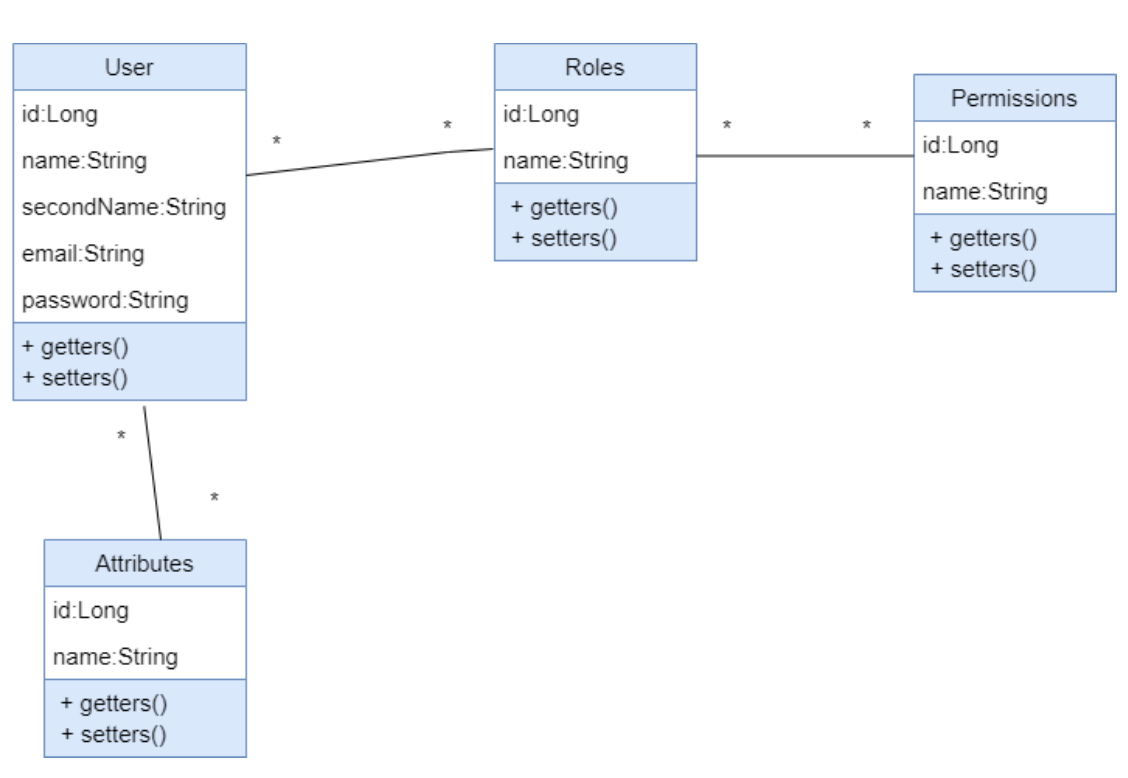
\includegraphics[width=16cm]{./chapters/sprint1/user_diagram.png}
  \caption{Manage users class diagram}
  \label{fig:diagram-class-manage_users}
\end{figure}

\subsection{Sequence diagram of "Authenticate" use case}

The following figure (\hyperref[fig:login_seq2]{Figure \ref{fig:login_seq2}})  represents the admin ``Authenticate'' sequence diagram.
\begin{figure}[h]
  \center
%\hspace*{-0.9in}
  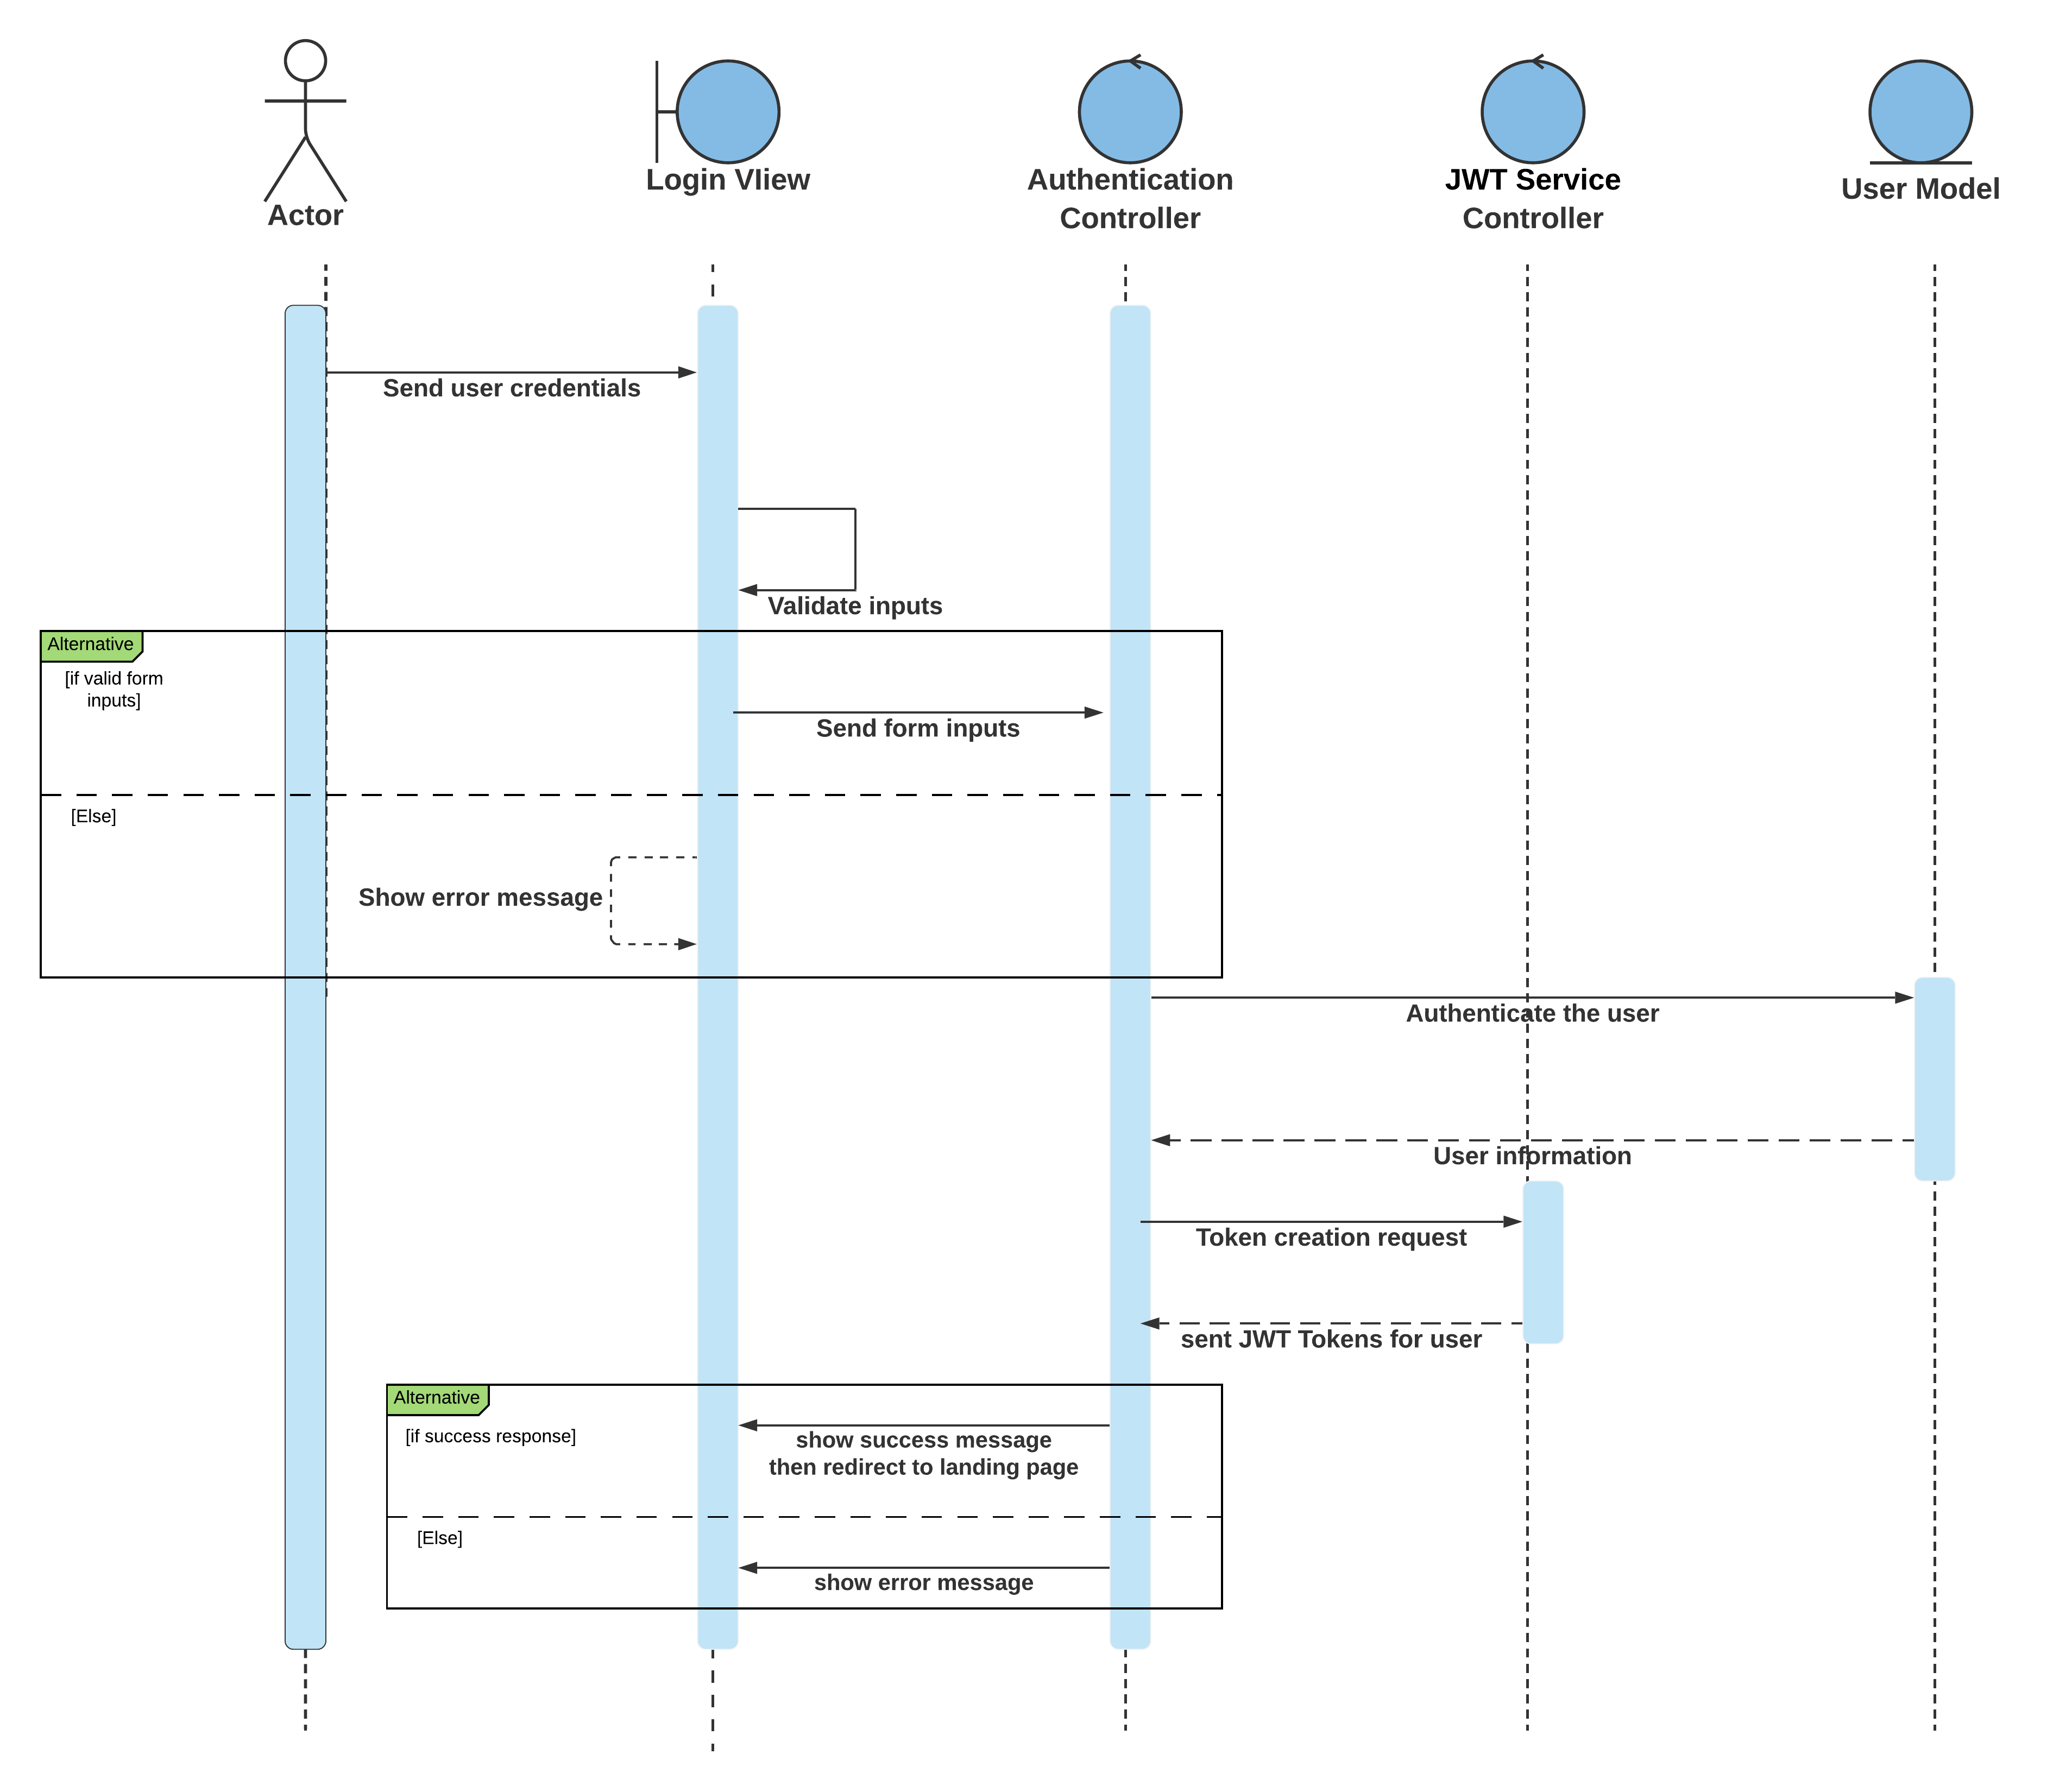
\includegraphics[width=14cm]{./chapters/sprint1/login_seq2.png}
  \caption{Sequence diagram: Authenticate}
  \label{fig:login_seq2}
\end{figure}
\vspace*{5cm}

\subsection{Use case diagram of "Manage Vault Secrets"}

The following figure (\hyperref[fig:use_case-manage_vault]{Figure \ref{fig:use_case-manage_vault}})  represents the ``Manage Vault Secrets'' detailed use case.
\begin{figure}[h]
  \center
%\hspace*{-0.9in}
  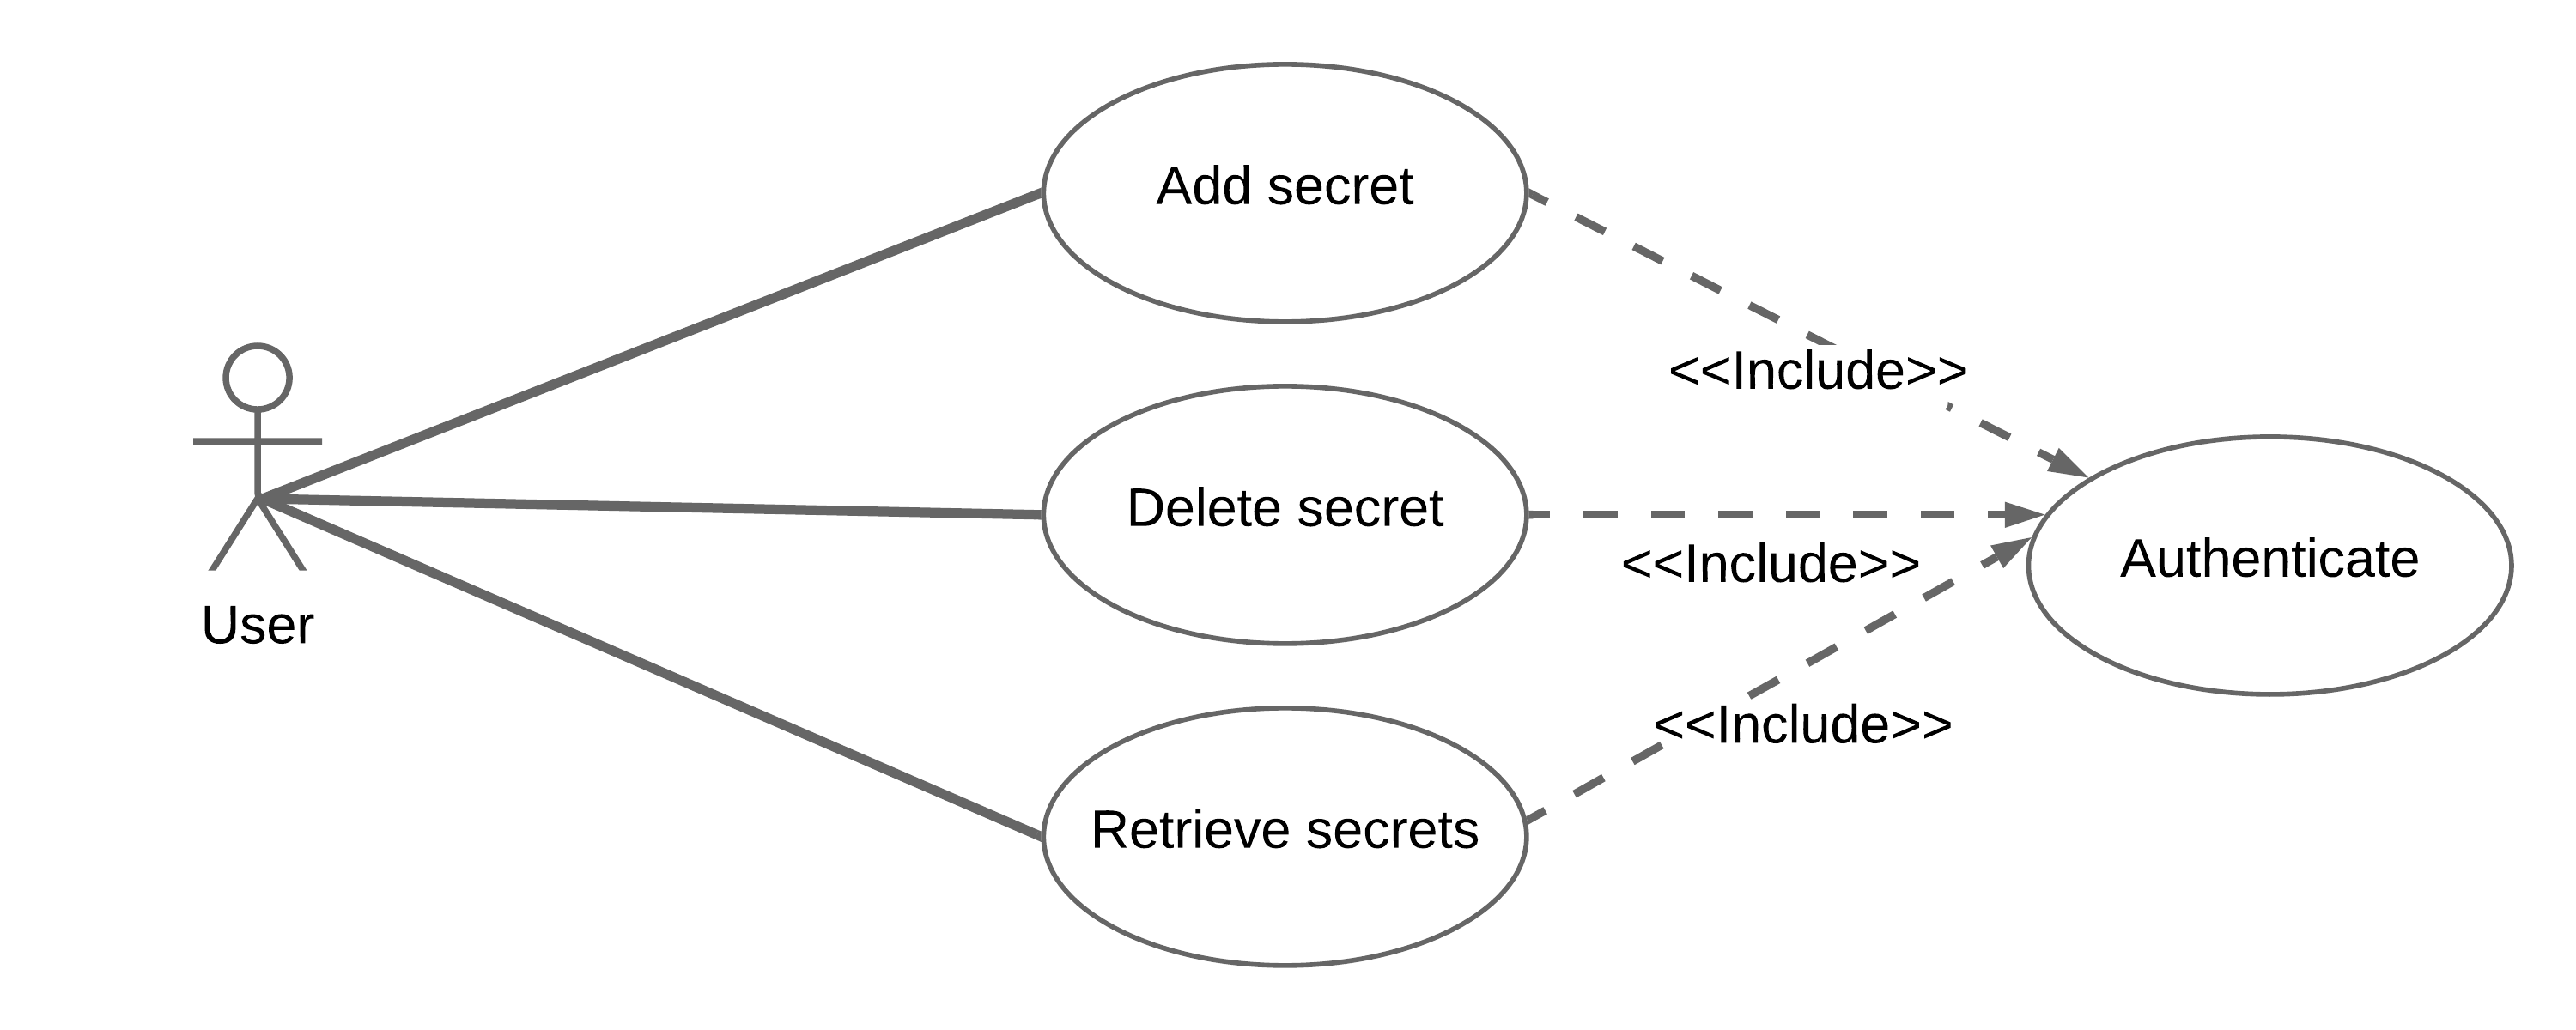
\includegraphics[width=14cm]{./chapters/sprint1/use_case-manage_vault.png}
  \caption{Vault Secrets detailed use case diagram}
  \label{fig:use_case-manage_vault}
\end{figure}
\vspace*{6cm}

\subsection{Interfaces}
In this section, we will provide some screenshots of our application interfaces. These screenshots will illustrate the various functionalities and processes related to user management as part of Sprint 1, as well as managing vault secrets. 

The following figure (\hyperref[fig:login_sprint]{Figure \ref{fig:login_sprint}})  depicts the login page of our application.
\begin{figure}[h]
  \center
%\hspace*{-0.9in}
  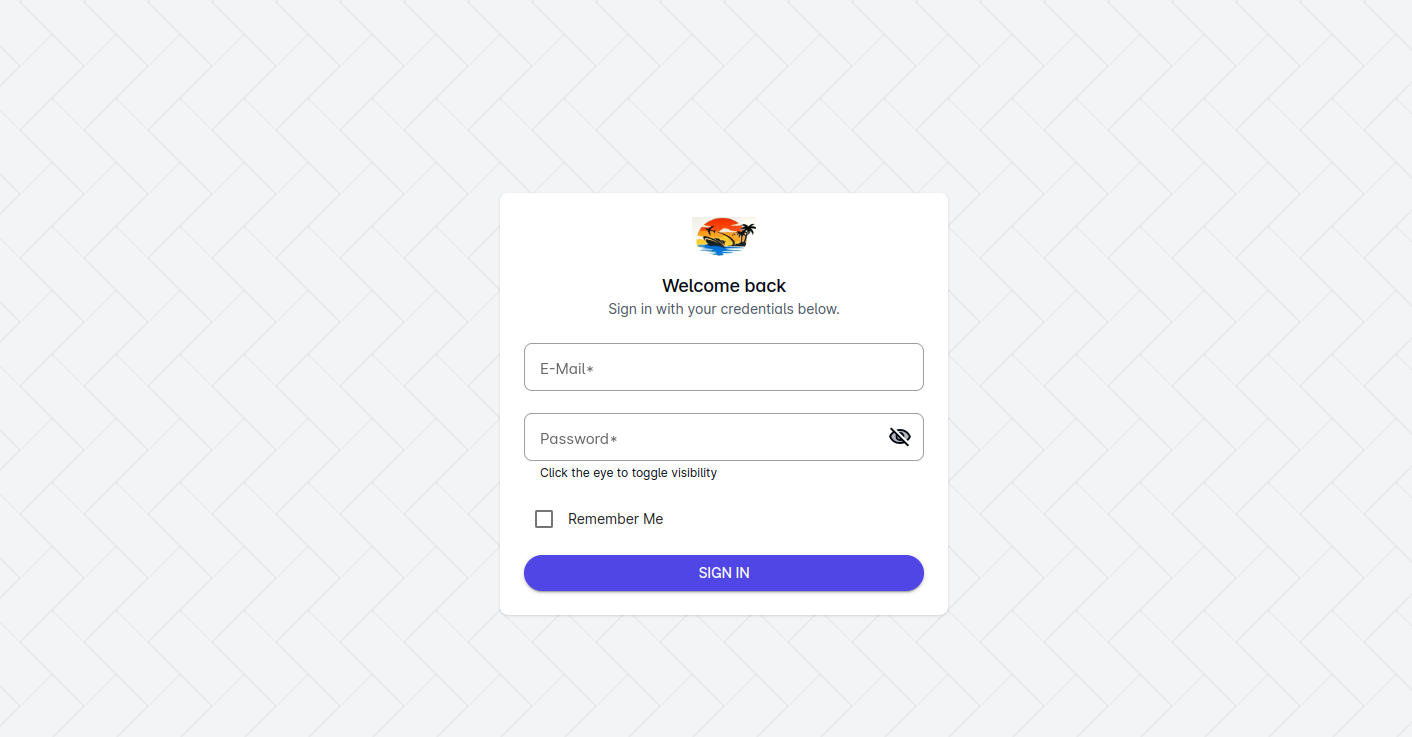
\includegraphics[width=14cm]{./chapters/sprint1/login.png}
  \caption{Ilef login page}
  \label{fig:login_sprint}
\end{figure}



The following figure (\hyperref[fig:add_user]{Figure \ref{fig:add_user}}) represents the User registration of our application.

\begin{figure}[h]
  \center
%\hspace*{-0.9in}
  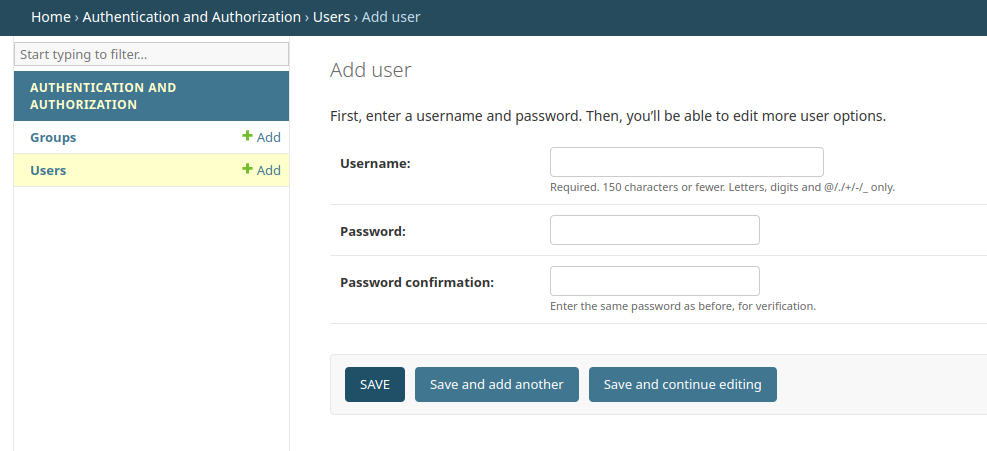
\includegraphics[width=15cm]{./chapters/sprint1/add_user.png}
  \caption{Ilef User registration page}
  \label{fig:add_user}
\end{figure}

The following figure (\hyperref[fig:vault_page]{Figure \ref{fig:vault_page}})  represents the Secret page of our application.
\begin{figure}[h]
  \center
%\hspace*{-0.9in}
  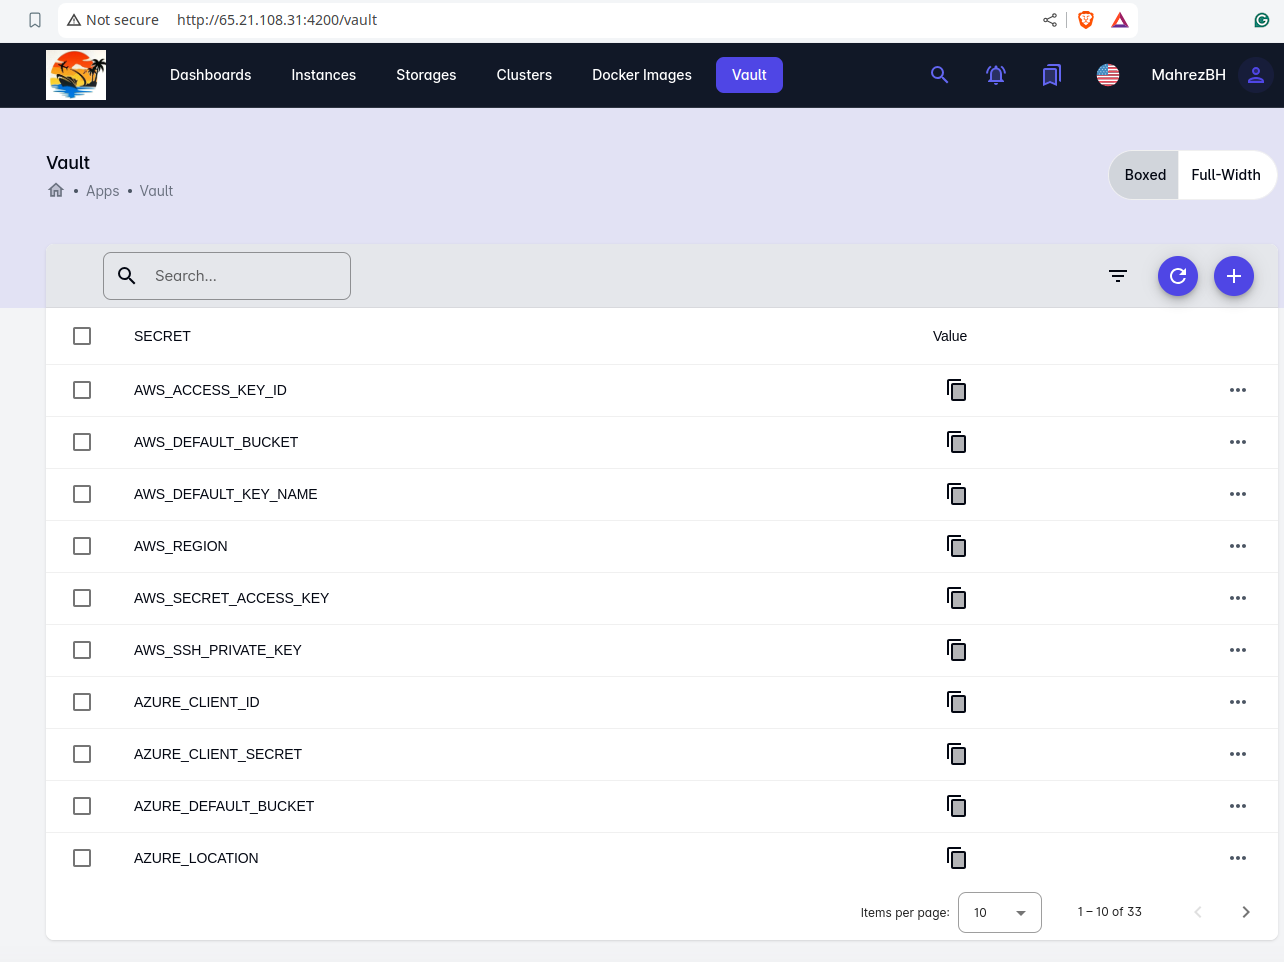
\includegraphics[width=15cm]{./chapters/sprint1/vault.png}
  \caption{Ilef adding User page}
  \label{fig:vault_page}
\end{figure}
\vspace*{15cm}

\section*{Conclusion}
This chapter includes various diagrams and screenshots from Sprint 1, showcasing the key functionalities and processes of our application, such as user management and the handling of vault secrets. These visual aids provide a comprehensive understanding of the development and implementation stages during Sprint 1.